
\documentclass[a4paper]{report}
% \documentclass{report}
\usepackage[utf8]{inputenc}
\usepackage{amsmath}
\usepackage{esint}
\usepackage{tabstackengine}
\usepackage[colorlinks,linkcolor=blue]{hyperref}
\usepackage{xeCJK}
\usepackage{caption}
\usepackage{stackengine}
\usepackage{graphicx}
\graphicspath{ {../resources/figure/infoTheory/} }
\usepackage{float}
\usepackage{amsmath}
\usepackage{ulem}
\usepackage{amsfonts}
\usepackage{blkarray}
\usepackage{enumitem}
\setlist[1]{itemsep=-5pt}
\usepackage{subcaption}

\usepackage{tikz}
\usetikzlibrary{calc}
\usepackage{pgfplots}
\usepackage{mathrsfs}
\usepackage{diagbox}
\usetikzlibrary{shapes,arrows,positioning}
\captionsetup[table]{skip=10pt}

%%%% 下面的命令重定义页面边距,使其符合中文刊物习惯 %%%%
\addtolength{\topmargin}{-54pt}
\setlength{\oddsidemargin}{0.63cm}  % 3.17cm - 1 inch
\setlength{\evensidemargin}{\oddsidemargin}
\setlength{\textwidth}{14.66cm}
\setlength{\textheight}{24.00cm}    % 24.62


% 段首不缩进
\setlength{\parindent}{0pt}
%%%% 下面的命令设置行间距与段落间距 %%%%
\linespread{1.2}
% \setlength{\parskip}{1ex}
\setlength{\parskip}{.5\baselineskip}

\def\rlwd{.5pt} \def\rlht{2.2ex} \def\rldp{.5ex}
\def\mydiv#1{~%
  \rule[-\rldp]{\rlwd}{\rlht}%
  \setbox0=\hbox{~#1}%
  \stackunder[\dimexpr\rldp-\rlwd]{~#1}{\rule{\wd0}{\rlwd}}%
}

\title{infoTheory}
\author{Crosstyan}
\date{Dec 2020}


\begin{document}
\chapter{Discrete Source and Entropy}
\section{Entropy}
\subsection{Self-Information}
随机事件的不确定度在数量上等于其自信息量
自信息在事件发生前表征时间不确定性的大小, 在事件发生后表征事件所提供的信息量

$I$里边的参数表征一个事件, 或者一个符号($x_i$)
\begin{align}
  I(x_i)&=\log_2{\frac{1}{p(x_i)}}\\
  &=-\log_2{p(x_i)}
\end{align}

\subsubsection{Property}
\begin{align*}
  p(x\mid y)=\frac{p(xy)}{p(y)} \Leftrightarrow  I(x\mid y)=I(xy)-I(y)\\
\end{align*}
\begin{align*}
  p(xy)&=p(x\mid y)\cdot p(y)\\
  &=p(y\mid x)\cdot p(x)\\
  &\Updownarrow\\
  I(xy)&=I(x\mid y)+I(y)\\
  &=I(y\mid x)+I(x)
\end{align*}

\subsection{Information Entropy}
信息熵表征
\begin{itemize}
  \item 信源输出前, 信源的平均不确定性. 
  \item 信源输出后, 每个消息(附后)所包含的平均信息量. 
  \item 信源, 即随机变量$\textbf{X}$的整体不确定度. 
\end{itemize}
$H$里面的参数是随机变量($\textbf{X}$), 或者是一堆概率(事件)(它们构成随机变量)

\begin{gather}
\begin{bmatrix}
  \textbf{X}\\\textbf{P}
\end{bmatrix}=
\begin{bmatrix}
  x_1 & x_2 & \dots & x_n\\
  p(x_1) & p(x_2)&\dots&p(x_n)
\end{bmatrix}
\end{gather}

\begin{align*}
  H(\textbf{X})=\displaystyle\sum_{i} p(x_i)\cdot\log{\frac{1}{p(x_i)}}
\end{align*}

\begin{gather}
  \begin{bmatrix}
    \textbf{X}\\\textbf{P}
  \end{bmatrix}=
  \begin{bmatrix}
    x_1 & x_2 \\
    p & 1-p
  \end{bmatrix}
  \Rightarrow 
  H(\textbf{X})=H(p,1-p)=H(p)
\end{gather}
\begin{align*}
  H(p)=p\cdot\log{\frac{1}{p}}+(1-p)\cdot\log{\frac{1}{1-p}}
\end{align*}

\subsubsection{条件熵}
\begin{align}
  H(Y\mid X)=\displaystyle\sum_{i=1}^{n} p(x_i)\cdot H(Y\mid x_i)
\end{align}

\paragraph{例如}给定联合概率矩阵和条件概率矩阵
\[
  P_{XY}=
\begin{blockarray}{cccc}
 &y_1 & y_2 & y_3  \\
\begin{block}{c[ccc]}
  x_1 & 1/8 & 1/8 & 0 \\
  x_2 & 0 & 1/4 & 1/2 \\
\end{block}
\end{blockarray}
 \]

\[
  P_{Y|X}=
\begin{blockarray}{cccc}
 &y_1 & y_2 & y_3  \\
\begin{block}{c[ccc]}
  x_1 & 1/2 & 1/2 & 0 \\
  x_2 & 0 & 1/3 & 2/3 \\
\end{block}
\end{blockarray}
 \]

 求联合熵$H(XY)$, 条件熵$H(Y\mid X)$

 可以求得$P_X$和$P_Y$
 \[
   P_X=
  \begin{bmatrix}
    \frac{1}{8}+\frac{1}{8}+0&0+\frac{1}{4}+\frac{1}{2}
  \end{bmatrix}\\
  =
    \begin{bmatrix}
    \frac{1}{4}&\frac{3}{4}
  \end{bmatrix}\\
   \]

 \[
   P_Y=
    \begin{bmatrix}
    \frac{1}{8}&\frac{3}{8}&\frac{1}{2}
  \end{bmatrix}\\
   \]

   当然更多时候是只给$P_{Y\mid X}$和$P_{X}$而后使用
   \begin{align}
    P_Y=P_X\cdot P_{Y\mid X}
   \end{align}
   $P_X,P_Y$均为行向量

 \begin{align*}
   H(XY)&=H(P_{XY}\text{矩阵里边的所有元素})\\
   &=H(0,\frac{1}{8},\frac{1}{8},0,\frac{1}{4},\frac{1}{2})\\
   &=H(\frac{1}{8},\frac{1}{8},\frac{1}{4},\frac{1}{2})\\
 \end{align*}
 \begin{align*}
  p(xy) &=p(y\mid x)\cdot p(x)
  \\   &\Downarrow 
  \\   H(XY)&=H(Y\mid X)+H(X)
  \\   &\Downarrow
  \\ H(Y\mid X) &=H(XY)-H(X)
 \end{align*}
 当然也可以用$P_X$和$P_{Y\mid X}$关系
 \begin{align*}
  H(Y\mid X)&=\displaystyle\sum_{i=1}^{n} p(x_i)\cdot H(Y\mid x_i)
  \\ &= \displaystyle\sum_{i=1}^{2} \text{$P_X$ 行向量每一个元素}\cdot H(\text{$P_{Y\mid X}$矩阵对应行元素})
  \\ &= \frac{1}{4}\cdot H(\frac{1}{2},\frac{1}{2},0)+\frac{3}{4}\cdot H(0,\frac{1}{3},\frac{2}{3})
 \end{align*}

\subsubsection{Property}
\paragraph{对称性}
两个信源, 只要发出的消息数相同, 概率分布相同, 则其信源熵必定相同
\paragraph{确定性}
只要有一个事件是必然事件, 那么其他事件必为不可能事件
$$H(1,0)=0$$
\paragraph{非负性}
$H(\textbf{X})\geq 0$ (仅对离散信源成立)
\paragraph{扩展性}
在概率空间中增加一个发生概率极小的随机事件, 信源熵保持不变
\paragraph{强可加性}
在信源$X$与信源$Y$相互关联时, 信源$XY$每发出一个符号组合所能提供的平均信息量, 
等于信源$X$每发出一个符号所能提供的平均信息量
再加上$X$在已知的条件下信源$Y$再发出一个符号所提供的平均信息量
\paragraph{上凸性}
信息熵是概率分布严格上凸函数
\paragraph{极值性}
等概时信息熵最大

\begin{align*}
  H(\textbf{XY})&=H(\textbf{X})+H(\textbf{Y}\mid \textbf{X})\\
  &=H(\textbf{Y})+H(\textbf{X}\mid \textbf{Y})
\end{align*}
当X和Y相互独立时
\begin{align*}
  H(XY)=H(X)+H(Y)
\end{align*}
N个变量相互独立时$H(X_1X_2\dots X_N)=\displaystyle\sum_{i=1}^{N}H(X_i)$, 
独立同分布时$H(X_1X_2\dots X_N)=N\cdot H(X_i)$

$H(X\mid Y)$条件熵, $H(XY)$联合熵较小
\begin{align*}
  \begin{cases}
    H(X\mid Y)\leq H(X)\\
    H(XY)\leq H(X)+H(Y)
  \end{cases}
\end{align*}





\section{Discrete Source}
\subsection{Discrete Stationary Source}
各维度条件概率只与关联长度有关, 与时间起点无关
\subsubsection{Entropy rate}
\begin{align*}
  H_\infty =H_{m+1}=H(\underset{\text{记忆长度}m+1}{X_{m+1}} \mid \underset{\text{条件概率阶数}m}{X_1X_2\dots X_m} )
\end{align*}
一般只会考记忆长度为2, 即只有前后两个符号之间有记忆
\begin{align*}
  H_\infty &=H_{2}=H(\underset{\text{记忆长度}}{X_{2}} \mid \underset{\text{条件概率阶数}}{X_1} )
  \\ &=\displaystyle\sum_{n}\underset{\text{一维分布概率}}{p(x_i)} \cdot H(\underset{\text{条件概率的每一行}}{X\mid x_i})
\end{align*}

\subsection{Markov Chain}
一堆状态, 随机变量的状态仅与上一时刻所处的状态所关联. 若Markov Chain的状态转移概率与初始时刻无关, 
则被称作齐次Markov Chain.

\subsubsection{求解稳态$W$}
对于齐次Markov Chain, \textbf{初始分布}以及\textbf{一步转移概率}能够描述整个Chain的统计特性. 
在步长足够大的情况下(趋于$\infty$), 最终各个状态的绝对概率分布会的达到\textbf{稳态} $W$. 

\begin{align*}
  \begin{cases}
    W\cdot P=W &\text{$P$为状态转移矩阵}\\ 
    \displaystyle\sum_{j} W_j=1 &W=[W_1 \; W_2 \; \dots \; W_N]\text{为转移到各个稳态的概率}
  \end{cases}
\end{align*}

\paragraph{例如}给定一个概率转移矩阵 (可能是符号, 也可能是状态)
\[
  P=
  \begin{bmatrix}
    0&0&1\\
    1/2&1/3&1/6\\
    1/2&1/2&0
  \end{bmatrix}
  \]求其稳态分布

  \[
  \begin{cases}
    W\cdot P=W \\
    \displaystyle\sum_{j} W_j=1
  \end{cases}
  \Rightarrow
  \begin{cases}
    \begin{bmatrix}
      W_1&W_2&W_3
    \end{bmatrix}
    \cdot 
      \begin{bmatrix}
    0&0&1\\
    1/2&1/3&1/6\\
    1/2&1/2&0
  \end{bmatrix}
    =
        \begin{bmatrix}
      W_1&W_2&W_3
    \end{bmatrix}
    \\
    W_1+W_2+W_3=1
  \end{cases}
\]
解线性方程组可以解出$W_1,W_2,W_3$

\subsubsection{Markov信源}
% 记忆长度为$M+1$时, 该时刻符号只依赖于前面$M$个符号(条件长度为$M$), 这样的信源就被称作$M$阶Markov信源. 
% 把时刻$i_1$到$i_m$的$m$个变量看作一个状态. 
\paragraph{例子}
假设二阶Markov信源, 其符号集
$X=\{0,1\}\Rightarrow$状态集$S=\{00,01,10,11\}$
转移概率
\begin{align*}
p(0\mid 00)&=p(1\mid 11)=0.8
\\ p(1\mid 00)&=p(0\mid 11)=0.2
\\ p(0\mid 01)&=p(1\mid 01)=p(0\mid 10)=p(1\mid 10)=0.5
\end{align*}
可以符号条件概率矩阵 
% \[
%   P(x\mid S_i)=
% \begin{blockarray}{cccc}
%  &y_1 & y_2 & y_3  \\
% \begin{block}{c[ccc]}
%   x_1 & 1/8 & 1/8 & 0 \\
%   x_2 & 0 & 1/4 & 1/2 \\
% \end{block}
% \end{blockarray}

%   \]
\[
  P(x\mid S_i)=
\begin{blockarray}{ccc}
 &x=0 & x=1   \\
\begin{block}{c[cc]}
  S_0=00 & 0.8 & 0.2  \\
  S_1=01 & 0.5 & 0.5  \\
  S_2=10 & 0.5 & 0.5  \\
  S_3=11 & 0.8 & 0.2  \\
\end{block}
\end{blockarray}
 \]
 状态转移矩阵 (row为条件)(求解最后到达的各个状态的稳态$W$使用此矩阵)
\[
  P(S_j\mid S_i)=
\begin{blockarray}{ccccc}
 &S_0=00 & S_1=01 &S_2=10&S_3=11  \\
\begin{block}{c[cccc]}
  S_0=00 & 0.8 & 0.2&0&0  \\
  S_1=01 &0&0& 0.5 & 0.5  \\
  S_2=10 & 0.5 & 0.5&0&0  \\
  S_3=11 &0&0& 0.8 & 0.2  \\
\end{block}
\end{blockarray}
 \]
两个矩阵大概是可以互推的. 假设三个连续符号序列

$$000\Leftrightarrow S_{00}\rightarrow S_{00} \Leftrightarrow S_{00}\rightarrow 0_{\text{symbol}}$$
$$001\Leftrightarrow S_{00}\rightarrow S_{01} \Leftrightarrow S_{00}\rightarrow 1_{\text{symbol}}$$
$$010\Leftrightarrow S_{01}\rightarrow S_{10} \Leftrightarrow S_{01}\rightarrow 0_{\text{symbol}}$$
$$\dots$$
$$111\Leftrightarrow S_{11}\rightarrow S_{11} \Leftrightarrow S_{11}\rightarrow 1_{\text{symbol}}$$


可知状态转移图如下
\begin{figure}[H]
\centering
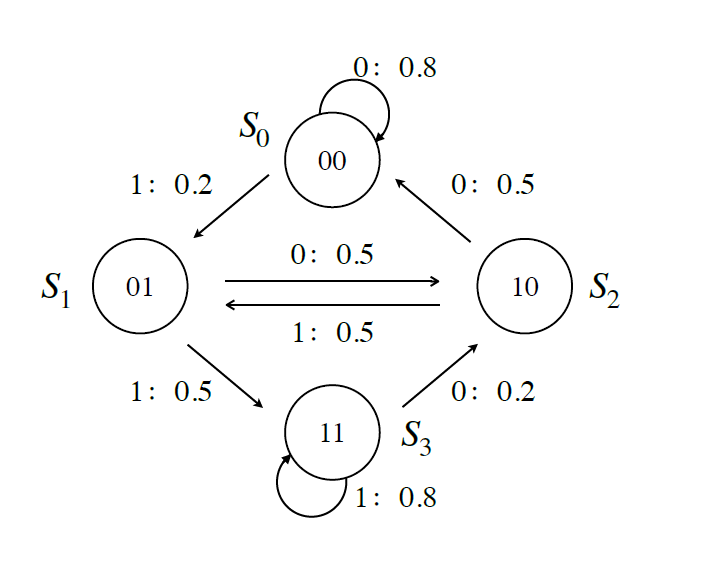
\includegraphics[width=0.5\textwidth]{markov.png}
\caption{二阶Markov状态转移图}
\end{figure}

使用状态转移矩阵来求解最后落到的状态的稳态

\[
  \begin{cases}
    \begin{bmatrix}
      W_1&W_2&W_3&W_4
    \end{bmatrix}
    \cdot 
      \begin{bmatrix}
   0.8 & 0.2&0&0  \\
  0&0& 0.5 & 0.5  \\
   0.5 & 0.5&0&0  \\
  0&0& 0.8 & 0.2  \\
  \end{bmatrix}
    =
        \begin{bmatrix}
      W_1&W_2&W_3&W_4
    \end{bmatrix}
    \\
    W_1+W_2+W_3+W_4=1
  \end{cases}
  \]

  解出$W$之后与符号转移矩阵相乘得到稳态时的最终符号概率 (符号的稳态分布)
  \[
        \begin{bmatrix}
      W_1&W_2&W_3&W_4
    \end{bmatrix}
    =
    \begin{bmatrix}
      p(00)&p(01)&p(10)&p(11)
    \end{bmatrix}
    \]
\[
    \begin{bmatrix}
      W_1&W_2&W_3&W_4
    \end{bmatrix}
    \cdot 
      \begin{bmatrix}
   0.8 & 0.2  \\
   0.5 & 0.5  \\
   0.5 & 0.5  \\
   0.8 & 0.2  \\
  \end{bmatrix}
    =
        \begin{bmatrix}
      p(0)&p(1)
    \end{bmatrix}
  \]



\subsubsection{Entropy rate}
Markov Chain的极限熵
使用\textbf{符号转移矩阵}和\textbf{状态的稳态}求解
\begin{align*}
  H_\infty (\vec{X})=\displaystyle\sum_{i}\underset{\text{每个状态的稳态概率}}{p(S_i)} \cdot H(\underset{\text{符号转移矩阵的每一行}}{symbol\mid S_i} )
\end{align*}
\subsection{Redundancy}
$H_0$好像是初始状态的信源熵? \\
熵的相对率$\eta=\frac{H_\infty}{H_0}$ \\
信源的冗余度$R=1-\frac{H_\infty}{H_0}=1-\eta$

\chapter{Channel and Channel Capacity}

\section{Entropy}
\paragraph{先验概率}$p(a_i)$
\paragraph{前向概率(传递概率)}$p(b_j\mid a_i)=p(y=b_j\mid x=a_i)$
\paragraph{后向概率(后验概率)}$p(a_i\mid b_j)=p(x=a_i\mid y=b_j)$
\paragraph{联合概率(后验概率)}$p(a_i b_j)=p(a_i)\cdot p(b_j\mid a_i)=p(b_j)\cdot p(a_i\mid b_j)$
\paragraph{输出符号概率}$P_Y=P_X\cdot P_{Y\mid X}$
\subsection{信道疑义度}
表示接收端收到信道输出的一个附后之后对信道输入的符号仍然存在的平均不确定性
\begin{align*}
  H(X\mid Y)=\displaystyle\sum_{j} p(y_j)\cdot H(X\mid y_j)
\end{align*}
\begin{itemize}
  \item 理想传输$H(X\mid Y)=0$ 已知输出对于输入没有不确定度
  \item 一般情况有$H(X\mid Y)< H(X)$ 表示收到输出之后对于输入的不确定度会减少
\end{itemize}

\subsection{Mutual Information}
表示事件$y_j$所给出的关于$x_i$的信息量. 
表示事件$y_j$出现前后关于$x_i$存在的不确定度的减少量. 
表示事件$y_j$出现后信宿获得的关于输入$x_i$的信息量. 
\begin{align}
  I(x_i;y_j)&=I(x_i)-I(x_i\mid y_j)
  \\ &=I(y_j)-I(y_j\mid x_i)
  \\ &=I(x_i)+I(y_j)-I(x_i y_j)
\end{align}
\subsubsection{Properties}
\paragraph{互易性}
$I(x_i;y_j)=I(y_j;x_i)$
\paragraph{可负性}
$$I(x_i;y_j)=\begin{cases}
  >0 &\text{正相关}\\
  =0 &\text{不相关(独立)}\\
  <0 &\text{负相关}\\
\end{cases}$$
\paragraph{互信息不可能大于其中一个事件的自信息}某事件的自信息是发生其他事件所能提供的关于该事件的最大信息量

\subsection{Average Mutual Information}
\textbf{随机变量}$X$和$Y$的平均互信息定义为\textbf{事件的互信息在联合概率空间中的统计平均}
\begin{align*}
  I(\textbf{X}\mid \textbf{Y})&=H(\textbf{X})-H(\textbf{X}\mid \textbf{Y})
  \\ &=H(\textbf{Y})-H(\textbf{Y}\mid \textbf{X})
  \\ &=H(\textbf{X})+H(\textbf{Y})-H(\textbf{XY})
\end{align*}
% \subsubsection{从输出端来看}
% \paragraph{信道疑义度/损失熵/后验熵}
% \paragraph{X的先验不确定度/先验熵/无条件熵}
% \paragraph{平均互信息}收到Y前后对于X的平均不确定度的减少量
% \subsubsection{从输入端来看}
% \paragraph{噪声熵}发出X后对随机变量Y存在的平均不确定度
% \paragraph{平均互信息}收到Y获得的信息量减去噪声引起的额外的信息量
\subsubsection{Properties}
\paragraph{非负性}互信息可负, 平均互信息非负$$I(X;Y)\geq 0$$ $X$与$Y$独立时等号成立
\paragraph{对称性} $I(X;Y)=I(Y;X)$
\paragraph{极值性} $I(X;Y)\leq \min\{H(X),H(Y)\}$
\paragraph{凸性定理}平均互信息时\textbf{输入信源概率分布}和\textbf{信道传递概率分布}的凸函数
\begin{itemize}
  \item 固定信道, 平均互信息是输入信源概率上凸函数, 有最佳输入分布, 使得平均互信息最大
  \item 固定信源, 平均互信息是信道传递概率下凸函数, 有最差信道, 干扰最大
\end{itemize}

\section{Channel and Channel Capacity}
\subsection{Definition}
\subsubsection{信息传输率}
又称码率, 信道中平均每个符号所传输的信息量. 
平均互信息$I(X;Y)$接收到Y之后平均获得的关于X的信息量. 
二者完全等价. 
$$R=I(X;Y)$$
\subsubsection{信息传输速率}
信道每秒钟平均传输的信息量, 单位bit/s
$$R_t=\frac{1}{t}\cdot I(X;Y)$$
\subsubsection{信道容量}
在最佳输入分布时, 最大信息传输率被定义为信道容量
$$C=\underset{p(x)}{\max} \{I(X;Y)\}$$
信道在单位时间内平均传输的最大信息量 (单位bit/s)
$$C_t=\frac{1}{t}\cdot C$$

\begin{itemize}
  \item 信道容量与信源的分布概率无关, 是完全描述信道统计特性的参量
  \item 信道容量是信道能够传输的最大信息率, 信道输入为最佳概率分布时, 信道的信息传输率刚好达到了该信道容量
\end{itemize}
\subsection{信道模型}
\subsubsection{Noiseless Lossless}
一对一, 单位阵
$$C=\log_2{\text{行数或列数}}$$
(单位阵行列相等)
\subsubsection{Noisy Lossless}
\begin{itemize}
  \item 一对多, 宽宽的, 输出多
  \item 损失熵为0, 互信息为$H(X)$
\end{itemize}
$$C=\log_2{\text{行数(输入符号个数)}}$$
\subsubsection{Lossy Noiseless}
\begin{itemize}
  \item 多对一, 高高的, 输入多
  \item 噪声熵为0, 互信息为$H(Y)$
\end{itemize}
$$C=\log_2{\text{列数(输出符号个数)}}$$
\subsection{Discrete Memoryless Channel}
% \paragraph{输入对称} 每一行由同一集合的诸元素排列而成
% \paragraph{输出对称} 每一列由同一集合的诸元素排列而成
\subsubsection{对称DMC}
行等于列
$$C=\log_2{\underset{\text{行数}}{r} }-H(\underset{\text{任意一行的元素}}{p_1,p_2,\dots ,p_n})$$
\paragraph{强对称(均匀)DMC}
对角线为$\bar{p}$, 其余元素为$\frac{p}{r-1}$

\subsubsection{准对称DMC}
按列(输出)划分出n个对称的子矩阵
$$C=\log_2{\underset{\text{行数}}{r} }
-H(\underset{\text{任意一行的元素}}{p_1,p_2,\dots ,p_n})
-\displaystyle\sum_{k=1}^{n}
\underset{\text{子矩阵行元素之和}}{N_k}\cdot
\log_2({\underset{\text{子元素列元素之和}}{M_k}})$$


\section{Continuous Channel Capacity}
香农公式
\begin{align*}
  C_t&=\underset{\text{Bandwidth}}{B}\cdot\log_2(1+\underset{\text{decimal}}{\text{SNR}})
  \\ \underset{\text{decimal}}{\text{SNR}}&=\frac{P_S}{P_N}=\frac{P_S}{N_0\cdot B}
  \\ \text{SNR}_{\text{dB}}&=10\cdot \lg(1+\underset{\text{decimal}}{\text{SNR}})
\end{align*}
$N_0$为噪声的单边功率谱密度

\chapter{
Information Rate-distortion Theory
}
压缩信源发出信息的冗余度. 在允许一定程度的失真的条件下, 能够把信源信息压缩到什么程度, 即最少需要多少比特才能描述信源

将信源编码和信源译码等价为一个信道, 
在\textbf{给定允许失真}的条件下, 设计一种信源编码使得\textbf{信息传输率R最低}
\section{Distortion functions}
信源分布为
\[
\begin{bmatrix}
  \textbf{X}\\\textbf{P}
\end{bmatrix}=
\begin{bmatrix}
  x_1 & x_2 & \dots & x_n\\
  p(x_1) & p(x_2)&\dots&p(x_n)
\end{bmatrix}
  \]
  输出$Y$为
  \[
    Y=\begin{bmatrix}
      y_1&y_2&\dots&y_m
    \end{bmatrix}
    \]

定义失真矩阵
\[
  D= \begin{bmatrix}
    d(x_1,y_1)&d(x_1,y_2)&\dots&d(x_1,y_m)\\
    d(x_2,y_1)&d(x_2,y_2)&\dots&d(x_2,y_m)\\
    \dots&\dots&\dots&\dots\\
    d(x_n,y_1)&d(x_n,y_2)&\dots&d(x_n,y_m)\\
  \end{bmatrix}
  \]


% \subsection{Hamming distortion}
% \subsection{Squared-error distortion}

\section{Rate–distortion functions}

率失真函数. 在限定失真$D$条件下的信源输出的最小信息速率

analytical expression不知道\dots
\paragraph{domain}平均失真度的取值范围$[0,D_{\max}]$
$$D_{\max}=\underset{j}{\min} \{ \displaystyle\sum_{i} p(x_i)\cdot d(x_i,y_j) \}$$
信源概率$p(x_i)$乘失真矩阵列元素求和, 取和最小一列. 
\paragraph{range}率失真函数的取值范围$[H(X),0]$
\begin{figure}[H]
\centering
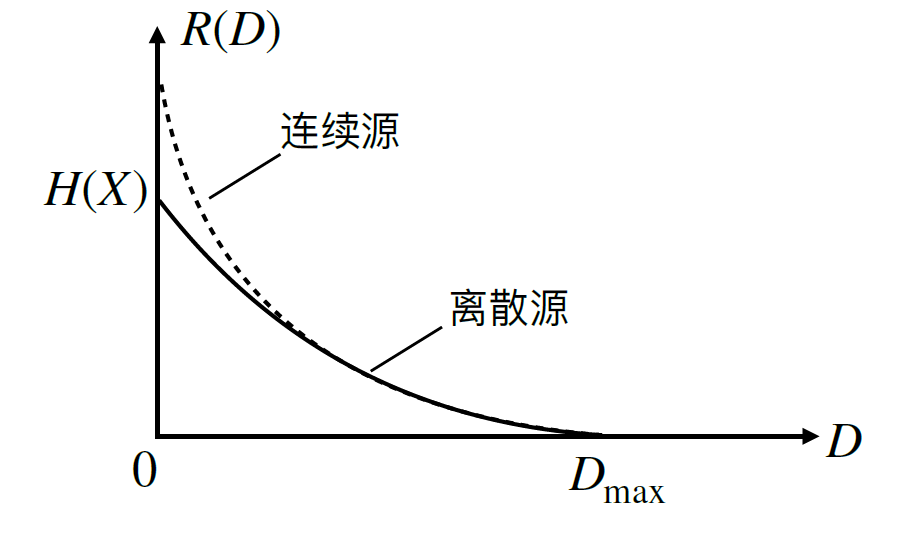
\includegraphics[width=0.5\textwidth]{rate_distortion.png}
\caption{率失真函数图像}
\end{figure}
\section{香农第三定理}
允许失真$D$的条件下, 信源最小可达的信息传输率是信源的$R(D)$, 提供了压缩的下界

\chapter{Source Coding}
无失真信源编码

\begin{figure}[H]
\centering
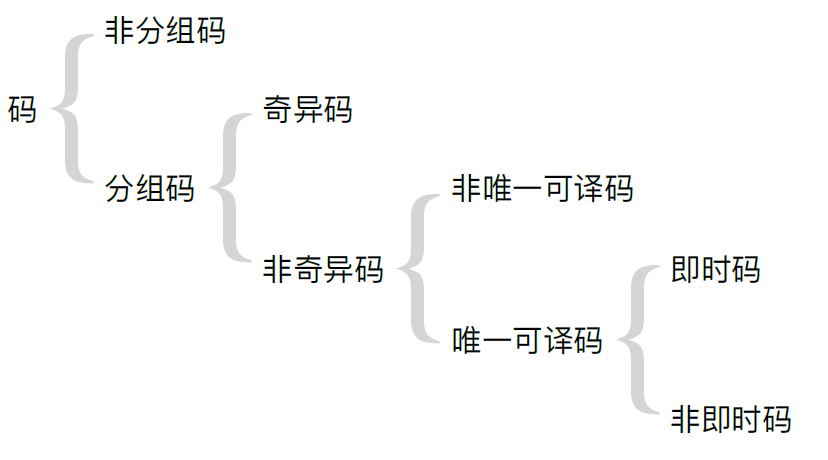
\includegraphics[width=0.5\textwidth]{source_coding_type.png}
\caption{信源编码分类}
\end{figure}
分组码好, 奇异码菜, 即时码必唯一可译
\section{唯一可译码的判定}
\section{Fixed-length Coding}
定长信源编码定理
\section{Variable-length Coding}
\subsection{Shannon coding}
\begin{itemize}
  \item 消息符号按其出现概率从大到小排列
  \item 对其概率取$\log_2$向上取整, 得到码长
  \item 对其\textbf{累加概率}转换为二进制, 取其为码字(长度为码长)
\end{itemize}
\subsection{Huffman Coding}
为了得到码方差最小的码, 应该使合并的信源符号位于缩减信源序列尽可能高的位置上, 以减小再次合并的次数, 充分利用短码



\chapter{Channel Coding}
有目的地增加一些监督码源, 增大了信息的冗余度, 以提高传输信息的可靠性. 
\section{译码规则}
\subsection{MAP}
最大后验概率
\begin{itemize}
  \item 转移矩阵每行乘以$p(x_i)$得到联合概率分布矩阵
  \item 以\textbf{联合概率分布矩阵}每\textbf{列}矩阵最大概率所对应的$x_i$作为译码准则
  \item $P_E=1-\displaystyle\sum_{i} \underset{\text{被选定为译码规则的联合概率}}{p(x_i y_j)}$
\end{itemize}
\subsection{ML}
最大似然概率
\begin{itemize}
  \item 输入符号为等概分布或者先验概率未知
  \item 以\textbf{转移概率矩阵}每\textbf{列}矩阵\textbf{最大概率所对应元素}所对应的$x_i$作为译码准则
  \item $P_E=1-\frac{1}{r}\cdot\sum_{i=1}^{r} \underset{\text{被选定为译码规则的转移概率}}{p(y_j|x_i)}$
\end{itemize}
\section{最小汉明距离}
The weight of a codeword is the number of its elements that are nonzero and the distance between two codewords is the Hamming distance between them, that is, the number of elements in which they differ. The distance d of the linear code is the minimum weight of its nonzero codewords, or equivalently, the minimum distance between distinct codewords. 

$$d_{\min}=\underset{\text{纠正错误个数}}{t}+\underset{\text{发现错误个数}}{l}+1\;\;\;(l>t)$$

\textbf{H}有$t$列线性无关, 且有$t+1$列线性相关. 则$$d_{\min}=t+1$$即最小码重为$t+1$
\section{Linear Block Code}
$k$ bit. $2^k$种不同信息(码组). 得到输出为$n$ bit的码字, 附加$r=n-k$ bit的校验码元

$$\underset{\text{校验bit个数}}{r}=\underset{\text{总码长}}{n}-\underset{\text{信息bit个数}}{k}$$
可以用
$$(\underset{\text{总码长}}{n},\underset{\text{信息bit个数}}{k})$$
代表一个线性分组码

以下加法为模二加\footnote{另一种考虑方式是不带进位的加法}(等同于XOR), 用+和$\oplus$将看心情混合使用. 

(7,3)线性分组码有7 bit长, 3 bit信息位. 若用$m_k$表示信息位, $c_i$表示校验位\footnote{也有用parity来表示校验的}则可以有: 某个校验位是多个信息位的XOR. 
通常题目会给出其等式关系. 如有线性分组码\footnote{$c_i$和$m_k$不一定混在一起}为$\vec{C}=[m_1,m_2,m_3,c_4,c_5,c_6,c_7]$及其校验位的不等式
\begin{align*}
  c_4&=m_1\oplus m_3
  \\c_5&=m_1\oplus m_2 \oplus m_3
  \\c_6&=m_1\oplus m_2
  \\c_7&=m_2\oplus m_3
\end{align*}
化简可以得到\footnote{XOR是不分加减的, 移过去仍然是XOR}
\begin{align*}
  m_1\oplus m_3\oplus c_4&=0
  \\m_1\oplus m_2 \oplus m_3\oplus c_5&=0
  \\m_1\oplus m_2\oplus c_6&=0
  \\m_2\oplus m_3\oplus c_7&=0
\end{align*}
将其写作矩阵的形式则有
\[
  \begin{bmatrix}
    1&0&1&1&0&0&0\\
    1&1&1&0&1&0&0\\
    1&1&0&0&0&1&0\\
    0&1&1&0&0&0&1
  \end{bmatrix}
  \cdot
  \begin{bmatrix}
    m_1\\m_2\\m_3\\c_4\\c_5\\c_6\\c_7
  \end{bmatrix}
  =
  \begin{bmatrix}
    0\\0\\0\\0
  \end{bmatrix}
\]
或者
$$\textbf{H}\cdot \vec{C}^T=\vec{0}$$
$\textbf{H}$为校验矩阵(Check Matrix)\footnote{矩阵是行$\times$列, 即整个校验矩阵为$(n-k)\times k$}, $\vec{C}$为码元向量. 若$\textbf{H}$满足
$$\textbf{H}=\begin{bmatrix}
  \underset{(n-k)\times k}{\textbf{P}^T}&\underset{\text{单位阵}(n-k)\times (n-k)}{\textbf{I}}
\end{bmatrix}$$
则$\textbf{H}$是一个系统化(标准)校验矩阵. 
若对$\textbf{H}$做一些变换可以得到生成矩阵(Generator Matrix)\footnote{生成矩阵$k\times n$}$\textbf{G}$
$$\textbf{G}=\begin{bmatrix}
  \underset{\text{单位阵}k\times k}{\textbf{I}}&\underset{k\times (n-k)}{\textbf{P}}
\end{bmatrix}$$
生成矩阵的每一行都是合法码字. 且有$\textbf{H}\cdot\textbf{G}^T=\vec{0}$
\subsection{Syndrome}
伴随式, 用于判断接收机的输入是否有错误, 如果有则纠正. 若有(7,3)码的校验矩阵
\[
  \textbf{H}=
    \begin{bmatrix}
    1&0&1&1&0&0&0\\
    1&1&1&0&1&0&0\\
    1&1&0&0&0&1&0\\
    0&1&1&0&0&0&1
  \end{bmatrix}
\]
判断
\[
  \vec{y_1}=
  \begin{bmatrix}
    1&0&1&0&0&1&1
  \end{bmatrix}
  \]

  \[
  \vec{y_2}=
  \begin{bmatrix}
    1&1&1&0&0&1&1
  \end{bmatrix}
\]

  \[
  \vec{y_3}=
  \begin{bmatrix}
    0&0&1&1&0&1&1
  \end{bmatrix}
  \]
是否有错误, 并纠错

\paragraph{解: }先求伴随式
$$\vec{s}^T=H\cdot \vec{y}^T$$得到
\[
  \vec{s_1}^T=
      \begin{bmatrix}
    1&0&1&1&0&0&0\\
    1&1&1&0&1&0&0\\
    1&1&0&0&0&1&0\\
    0&1&1&0&0&0&1
  \end{bmatrix}\cdot 
    \begin{bmatrix}
    1\\0\\1\\0\\0\\1\\1
  \end{bmatrix}
\]

取$\textbf{H}$的第一行与$\vec{y_1}^T$相乘
\begin{equation*}\begin{array}{c}
\phantom{\times}1011000\\
\underline{\times1010011}\\
\phantom\times 1010000
\end{array}\end{equation*}
然后再对相乘的结果模二加(XOR)\footnote{以下用$\sum_\oplus$来表示, 当然这不是一个正式的表示, 只是我自己觉得这样写很爽. 如果里面有奇数个1, 那就是1; 如果为偶数个1, 那就是0. (严格意义来说应该是对每一位进行XOR)}, 得到伴随式$\vec{s_1}^T$的第一行
$$\displaystyle\sum_{\oplus}(1010000)=0=s_{1_1}$$
同理可得其余$\vec{s_1}^T$的行都为0. 即$\vec{s_1}=[0,0,0,0]$, 即没有错误. 

让我们来看看$\vec{y_2}$是否有错误
\[
  \vec{s_2}^T=
      \begin{bmatrix}
    1&0&1&1&0&0&0\\
    1&1&1&0&1&0&0\\
    1&1&0&0&0&1&0\\
    0&1&1&0&0&0&1
  \end{bmatrix}\cdot 
    \begin{bmatrix}
    1\\1\\1\\0\\0\\1\\1
  \end{bmatrix}
\]
取$\textbf{H}$的各行与$\vec{y_2}^T$相乘
\begin{equation*}\begin{array}{c}
\phantom{\times}1011000\\
\underline{\times1110011}\\
\phantom\times \sum_{\oplus} 1010000=0
\end{array}\end{equation*}

\begin{equation*}\begin{array}{c}
\phantom{\times}1110100\\
\underline{\times1110011}\\
\phantom\times \sum_{\oplus} 1110000=1
\end{array}\end{equation*}

\begin{equation*}\begin{array}{c}
\phantom{\times}1100010\\
\underline{\times1110011}\\
\phantom\times \sum_{\oplus} 1100001=1
\end{array}\end{equation*}

\begin{equation*}\begin{array}{c}
\phantom{\times}0110001\\
\underline{\times1110011}\\
\phantom\times \sum_{\oplus} 0110001=1
\end{array}\end{equation*}
则有
\[
  \vec{s_2}^T=
  \begin{bmatrix}
    0\\1\\1\\1
  \end{bmatrix}
  \]
看看和$\textbf{H}$中的第几\textbf{列}相同, 那就是第几位错. 在这里与$\textbf{H}$的第二列相同, 故纠错为$y_2=1110011$

类似, $y_3$得到的
\[
  \vec{s_2}^T=
  \begin{bmatrix}
    0\\1\\1\\0
  \end{bmatrix}
  \]
  并不是\textbf{H}中的任何一列, 表明错码大于1个. 有多种纠错可能. 

\subsection{Hamming code}
汉明码, 仅纠正单个错误. 
\begin{itemize}
  \item 有$r$个校验位 ($r=n-k$)
  \item 码长为$n=2^r-1$
  \item 信息位为$k=n-k$
\end{itemize}
常见的有(3,1), (7,4), (15, 11)\footnote{分别取$r=2,3,4$}汉明码

\paragraph{构造方式: }将$r$ bit按照二进制排序(除去最开始的全0码字), 得到$2^r-1$种组合, 塞到\textbf{H}矩阵的列里面. 以(7,4)汉明码为例则是
\[
  \textbf{H}=
  \begin{bmatrix}
    0&0&0&1&1&1&1\\
    0&1&1&0&0&1&1\\
    1&0&1&0&1&0&1
  \end{bmatrix}
  \]
注意观察矩阵的列, 别看行, 行没用. 

这时候我们得到的是一个非标准化的\textbf{H}, 需要化成标准化的$\textbf{H}=[\textbf{P}^T \quad \textbf{I}_{(n-k)}]$
可以选择直接列置换(交换某些列得到) 使得最后三列为单位阵\footnote{$c_1\leftrightarrow c_7,c_2\leftrightarrow c_6, c_4\leftrightarrow c_5$}
% \[
%   \textbf{H}=
%   \begin{bmatrix}
    
%   \end{bmatrix}
%   \]

\subsection{cyclic code}
循环码中任意一许用码经过循环移位后得到的码组仍然为许用码. 
题目往往会给你一个生成多项式$g(x)$, 其中的$x$并没有实际意义, 而其指数代表码字移位(or something else)

\subsubsection{码多项式}
用多项式来表示二进制符号
% Table generated by Excel2LaTeX from sheet 'Sheet1'
\begin{table}[H]
  \centering
  \caption{码字和码多项式关系}
    \begin{tabular}{cc}
    码字    & 多项式 \\
    000   & $0$ \\
    001   & $1$ \\
    010   & $x$ \\
    011   & $x+1$ \\
    100   & $x^2$ \\
    101   & $x^2+1$ \\
    110   & $x^2+x$ \\
    111   & $x^2+x+1$ \\
    \end{tabular}
\end{table}

\begin{itemize}
  \item 乘上$x^i$: 左移$i$位
  \item 加减法: 其系数若为偶数则相当于为0 (相当于不进位加法)
  \item 乘除法: 模二加 (XOR) $\oplus$
\end{itemize}


\subsubsection{构造生成矩阵(Generator Matrix)方法}
\paragraph{非典型(非系统)生成矩阵}
别忘了生成矩阵是$k\times n$的矩阵
\begin{gather}
  \textbf{G}=
  \begin{bmatrix}
    x^{k-1}\cdot g(x)
    \\x^{k-2}\cdot g(x)
    \\ \dots
    \\ x\cdot g(x)
    \\ g(x)
  \end{bmatrix}
\end{gather}
对其做行变换(万万不可做列变换)就可以得到系统生成矩阵\footnote{或者直接rref()}
\paragraph{给定某个消息码求出对应的码矢(输出)}
一个码矢, 等于消息位加校验位
$$c(x)=\underset{\text{消息位}}{m(x)}+\underset{\text{校验位}}{r(x)} $$
$$r(x)=(m(x)\cdot x^{n-k})\quad  \text{mod} \quad g(x)$$
即$m(x)\cdot x^{n-k}$之后再对$g(x)$求模. 与其说是多项式除法倒不如说是二进制除法. (只考虑位数即可, 多项式除法的系数不需要考虑, 相减相当于做XOR) \footnote{可以直接由CAS的expand()直接得出? 不太靠谱}
\paragraph{例子}
已知编码率为$\frac{1}{3}, $设生成多项式$g(x)=x^{10}+x^8+x^5+x^4+x^2+x^1+1$求消息多项式$m(x)=x^4+x+1$编为系统码之后的码多项式. 

编码率为$\frac{1}{3}$可以得到$n$(总码长)与$k$(信息位码长)的关系, 生成多项式的最高次幂又给出了$n-k$
$$\begin{cases}
  \frac{k}{n}=\frac{1}{3}\\
  n-k=10
\end{cases}
$$
可以得到$n=15,k=5,n-k=10$
$$m(x)\cdot x^{n-k}=x^{14}+x^{11}+x^{10}$$
问题在求$m(x)\cdot x^{n-k}\, \text{mod} \, g(x)$, 将$x$的幂次看作是码中为$1$的对应位数则可以列竖式. \footnote{严格来说应该是对应二进制位数对齐的, 可是这里十几位看得眼都花了, 不如直接标出位数然后做XOR}
\begin{figure}[H]
\centering
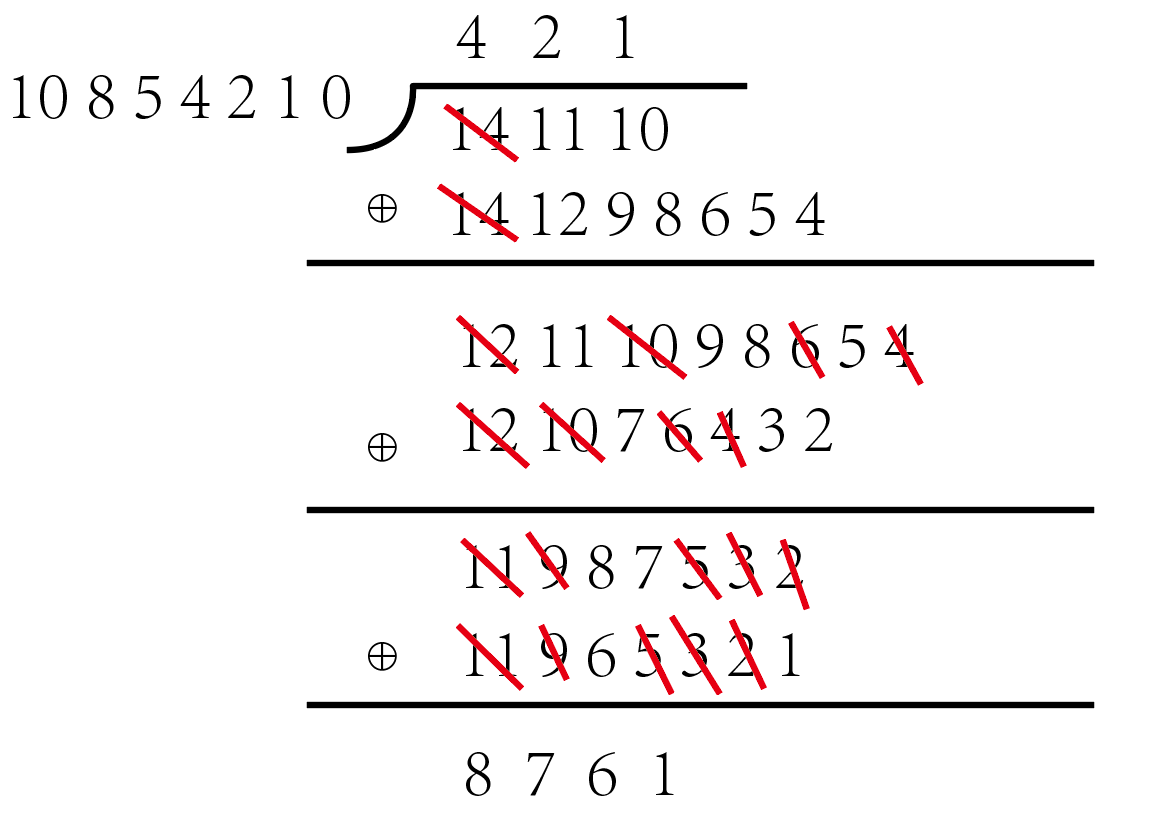
\includegraphics[width=0.33\textwidth]{mod2.png}
\caption{多项式模二除法}
\end{figure}
得到$r(x)=x^8+x^7+x^6+x$, 故$c(x)=m(x)+r(x)=x^{14}+x^{11}+x^8+x^7+x^6+x$

要得到标准化的矩阵$\textbf{G}$就利用
\[
  \textbf{G}=
  \begin{bmatrix}
    x^{n-1}+r_1(x)\\
    x^{n-2}+r_2(x)\\
    \dots\\
    x^{n-k}+r_k(x)
  \end{bmatrix}
  \]
  其中$$\begin{cases}
    r_1=x^{n-1}\quad\text{mod}\quad g(x)\\
    r_2=x^{n-2}\quad\text{mod}\quad g(x)\\
    \dots\\
    r_k=x^{n-k}\quad \text{mod}\quad g(x)\\
  \end{cases}$$

\section{卷积码}
\paragraph{(N,K,L)} $N$为$c_i$个数(编码器图中加法器的个数), 
$K$是编码器输入时有几种选择方向, 即有几组分组, 且是它是转移函数矩阵的行数(一般为1), 
$L+1$就是编码器图里面的序列长度$m^{i}$, 且是转移函数矩阵的列数
% $N$为分组码长, $K$为分割长度, $L+1$为约束长度\footnote{某一时刻的编码输出取决于本时刻的分组和本时刻以前的$L$个分组}

% $(N,K)$卷积编码器可以类比一个有$K$输入, $N$输出的多端口网络, 
% $K\times N $多项式矩阵$G(D)$中的元素$g_{kn}(D)$描述了第$k$行输入对第$n$列输出码元的影响, 
% 类似于多端口网络第$k$输入端对第$n$输入端的影响. 把$G(D)$定义为转移函数矩阵. 

% 转移函数矩阵$G(D)$给定, 卷积编码器的结构亦确定
\paragraph{转移函数矩阵}
一般只考$K=1$. 也就是只有一行. 
例如
$$\textbf{G}(D)=\begin{bmatrix}
  \underset{c_0^i}{1}&\underset{c_1^i}{1+D}&\underset{c_2^i}{1+D+D^2}
\end{bmatrix}$$
每列代表一个$c^i$, 而$D$代表延时, $D^n$等价于$m^{i-n}$. 这样一个矩阵可以写作
$$\begin{cases}
  c_0^i=m^i
  \\c_1^i=m^i+m^{i-1}
  \\c_2^i=m^i+m^{i-1}+m^{i-2}
\end{cases}$$
\paragraph{状态流图}
第一步定义状态$S^i$与$m^{i-1}$和$m^{i-2}$的关系, 这是定死的. 
\begin{table}[H]
  \centering
\begin{tabular}{|l|cc|}
   \hline
   \diagbox{状态}{$m^{i-n}$} & $m^{i-1}$ & $m^{i-2}$  \\
   \hline
   $S_0$ & 0 & 0  \\
   $S_1$  & 0 & 1 \\
   $S_2$  & 1 & 0 \\
   $S_3$  & 1 & 1 \\
   \hline
\end{tabular}
\caption{编码器状态定义}
\end{table}
第二步定义本状态$S^i$与下一状态$S^{i+1}$与输入$m^i$关系(定死的). 在当前状态下的左边插一个输入$m_{i}$组合成为$m_i\, m^{i-1} \, m^{i-2}$, 从左到右的两位成为新的状态. 
\begin{table}[H]
  \centering
\begin{tabular}{|l|cc|}
   \hline
   \diagbox{状态}{次态}{输入} & $m^{i}=0$ & $m^{i}=1$  \\
   \hline
   $S_0(00)$ & $\underset{\underline{00}0}{S_0}$ & $\underset{\underline{10}0}{S_2}$  \\
   $S_1(01)$  & $\underset{\underline{00}1}{S_0}$ &$\underset{\underline{10}1}{S_2}$  \\
   $S_2(10)$  & $\underset{\underline{01}0}{S_1}$ & $\underset{\underline{11}0}{S_3}$ \\
   $S_3(11)$  & $\underset{\underline{01}1}{S_1}$ & $\underset{\underline{11}1}{S_3}$ \\
   \hline
\end{tabular}
\caption{状态转移(随着输入$m^i$)}
\end{table}
第三步, 到这里不能背书了, 因为这与$\textbf{G}(D)$有关
\begin{align*}
  \text{码字}&=f(S^i,m^i)
  \\ &=f(m^{i},m^{i-1},m^{i-2})
  \\ &=c_0^i\; c_1^i\; c_2^i
\end{align*}

每个$S_n(m^{i-1}\; m^{i-2})$之中隐含着$m^{i-1},m^{i-2}$(由编码器状态定义给出), 再加上输入$m_i=0$就可以算出码字\footnote{模二加, 注意是模二加}(按列来看, 按列来看!) 其中$m_i=1$就是对$m_i=0$的码字取反, 不用再算一遍啦! 
$$\begin{cases}
  c_0^i=m^i
  \\c_1^i=m^i+m^{i-1}
  \\c_2^i=m^i+m^{i-1}+m^{i-2}
\end{cases}$$

算完可以得到以下表格

% Table generated by Excel2LaTeX from sheet 'Sheet1'
\begin{table}[H]
  \centering
    \begin{tabular}{|c|ccc|ccc|}
      \hline
    输入 & \multicolumn{3}{c|}{$m_i=0$} & \multicolumn{3}{c|}{$m_i=1$} \\
    \hline
    码字 & $c_0^i$    & $c_1^i$   & $c_2^i$   & $c_0^i$   &  $c_1^i$   &  $c_2^i$\\
    \hline
    $S_0(00)$    &   0    &  0     &  0     &   1    &   1    & 1 \\
    $S_1(01)$    &   0    &  0     &  1     &   1    &   1    & 0 \\
    $S_2(10)$    &   0    &  1     &  1     &   1    &   0    & 0 \\
    $S_3(11)$    &   0    &  1     &  0     &   1    &  0     & 1 \\
    \hline
    \end{tabular}%
  \caption{不同状态对应的输出码字}
\end{table}%

以$S_2$状态$m_i=0$为例. $S_2\Rightarrow m^{i-1}=1,m^{i-2}=0$. 
$$\begin{cases}
  c_0^i=m^i=0
  \\c_1^i=m^i+m^{i-1}=0\oplus 1=1
  \\c_2^i=m^i+m^{i-1}+m^{i-2}=0\oplus 1\oplus 0=1
\end{cases}$$

之后就可以画状态转移图了, 其中横向上写
$$S_1\rightarrow S_0$$
$$\underset{\text{箭头始端状态的输入}}{0} / \underset{\text{箭头始端状态的码字}}{011}$$



\paragraph{网格图(篱笆图)}
最上面的一条为全0信息/输出全0码字时的路径. 
最短汉明距离为
\begin{quotation}
  $S_0$状态转移回$S_0$状态所走的路径所用的最小码重(码字中为1的个数)
\end{quotation}
(当然不算最上面的参考距离)

当然也可以用来找特定输入序列得到的输出码字



\chapter{Encryption}
\section{RSA}
题目会给$p,q$和加密密钥$e$, 求解密密钥$d$并加密$x$为某个数. 

$(e,n)$为公钥, $(d,n)$为私钥, $y$为密文$x$为明文
\begin{itemize}
  \item $n=p\cdot q$
  \item 欧拉函数$\Phi(n)=(p-1)\cdot (q-1)$
  \item 解$(e\cdot d)\quad \text{mod} \quad \Phi(n)=1$求出$d$ (重点! )
  \item 加密 $y=x^e \quad \text{mod}\quad n$
  \item 解密 $x=y^d \quad\text{mod}\quad n$
\end{itemize}

\end{document}